\newcommand{\figwidth}{0.49\textwidth}
\begin{figure}[H]
	\centering
	\begin{subfigure}[b]{\figwidth}
		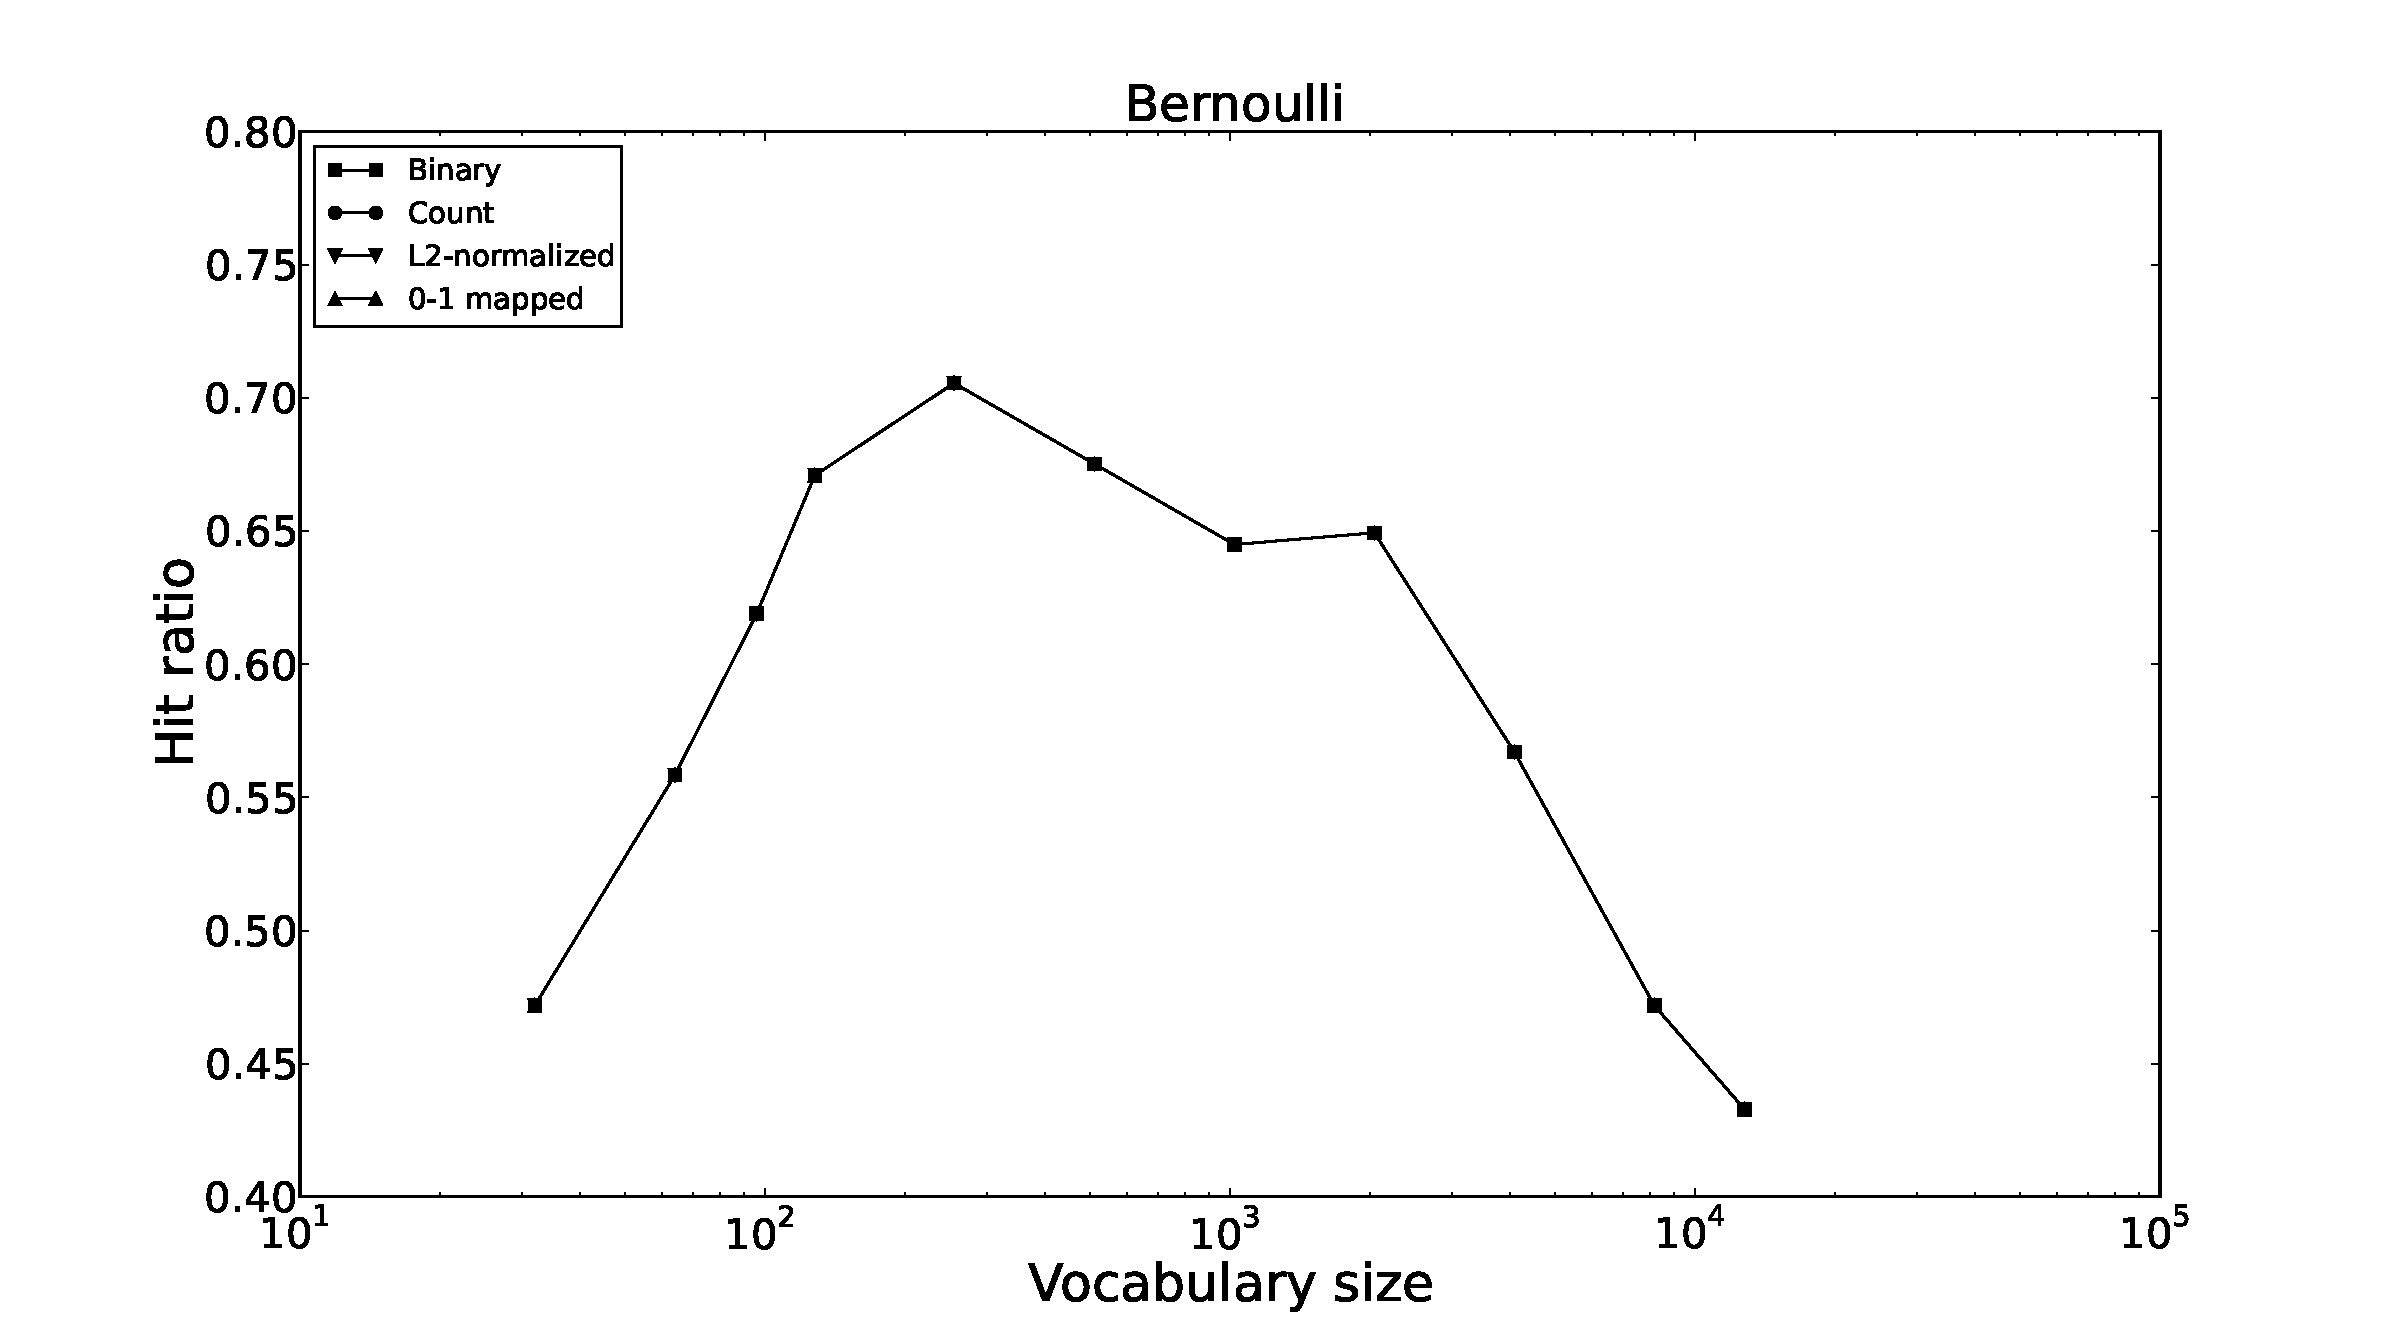
\includegraphics[width=\textwidth]{img/Bernoulli-hitrate-eps-converted-to.pdf}
		\caption{Hit ratio of Bernoulli classifier with varying vocabulary size. All values greater than zero are mapped to one, hence the different data types result in same accuracy.}
		\label{fig:hitratio-nb}
	\end{subfigure}
	~
	\begin{subfigure}[b]{\figwidth}
		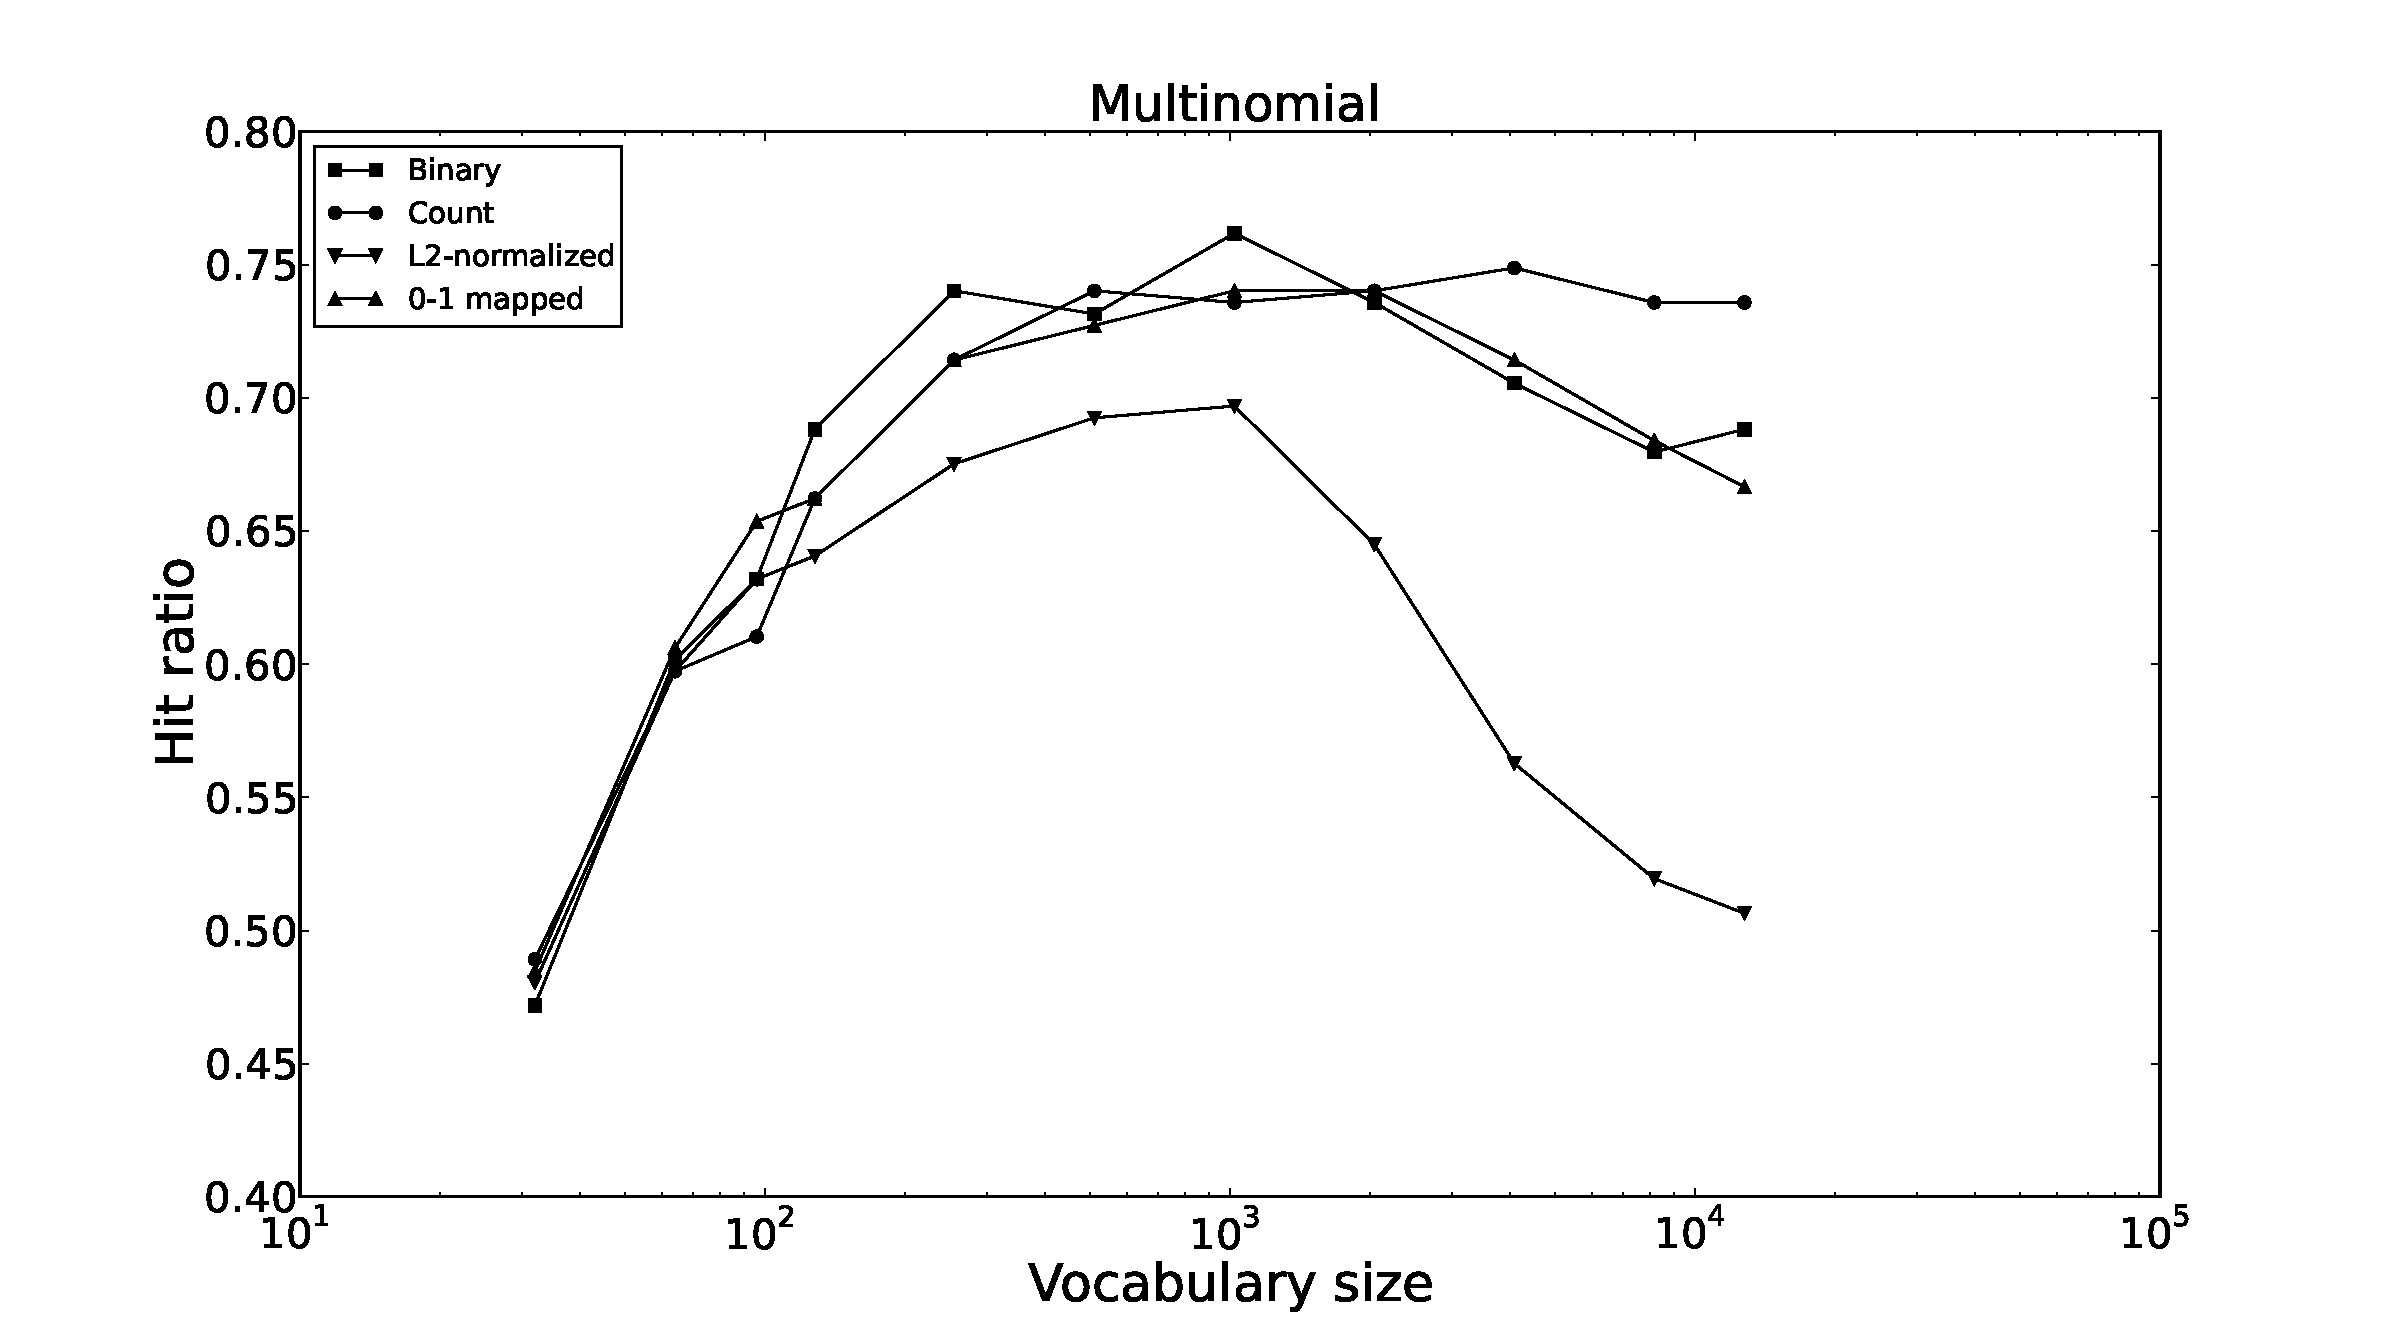
\includegraphics[width=\textwidth]{img/Multinomial-hitrate-eps-converted-to.pdf}
		\caption{Hit ratio of Multinomial classifier with varying vocabulary size.\\\ \\\ }
		\label{fig:hitratio-mn}
	\end{subfigure}
	\\
	\begin{subfigure}[b]{\figwidth}
		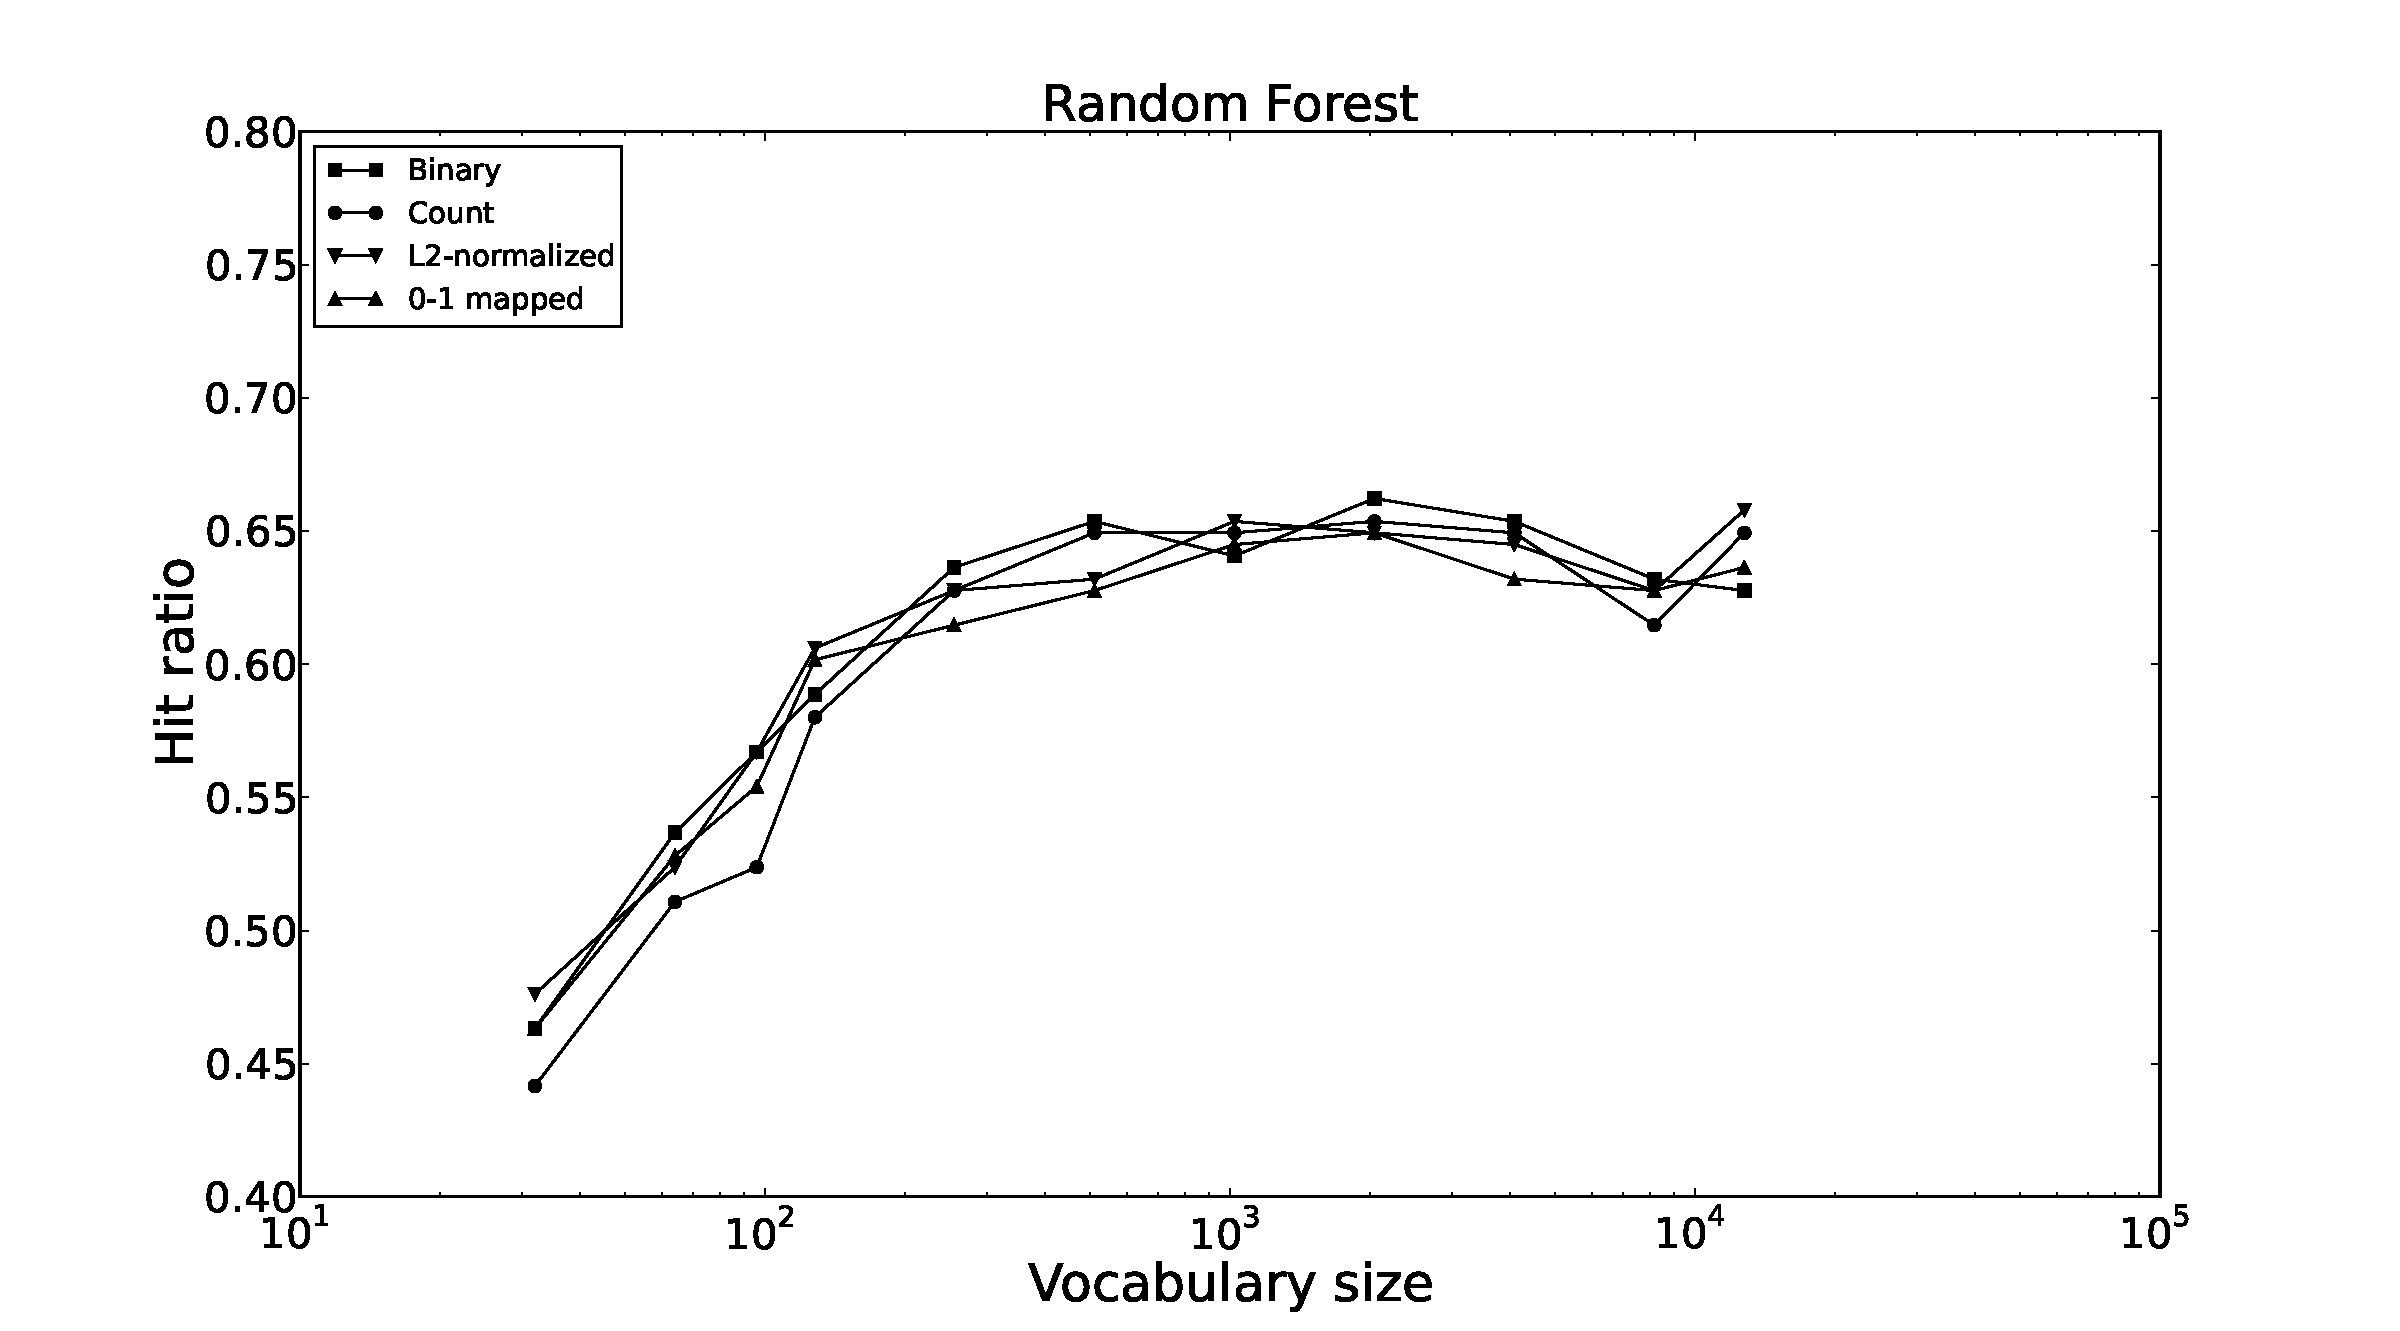
\includegraphics[width=\textwidth]{img/Random-Forest-hitrate-eps-converted-to.pdf}
		\caption{Hit ratio of Random Forest classifier with varying vocabulary size.}
		\label{fig:hitratio-rf}
	\end{subfigure}
	~
	\begin{subfigure}[b]{\figwidth}
		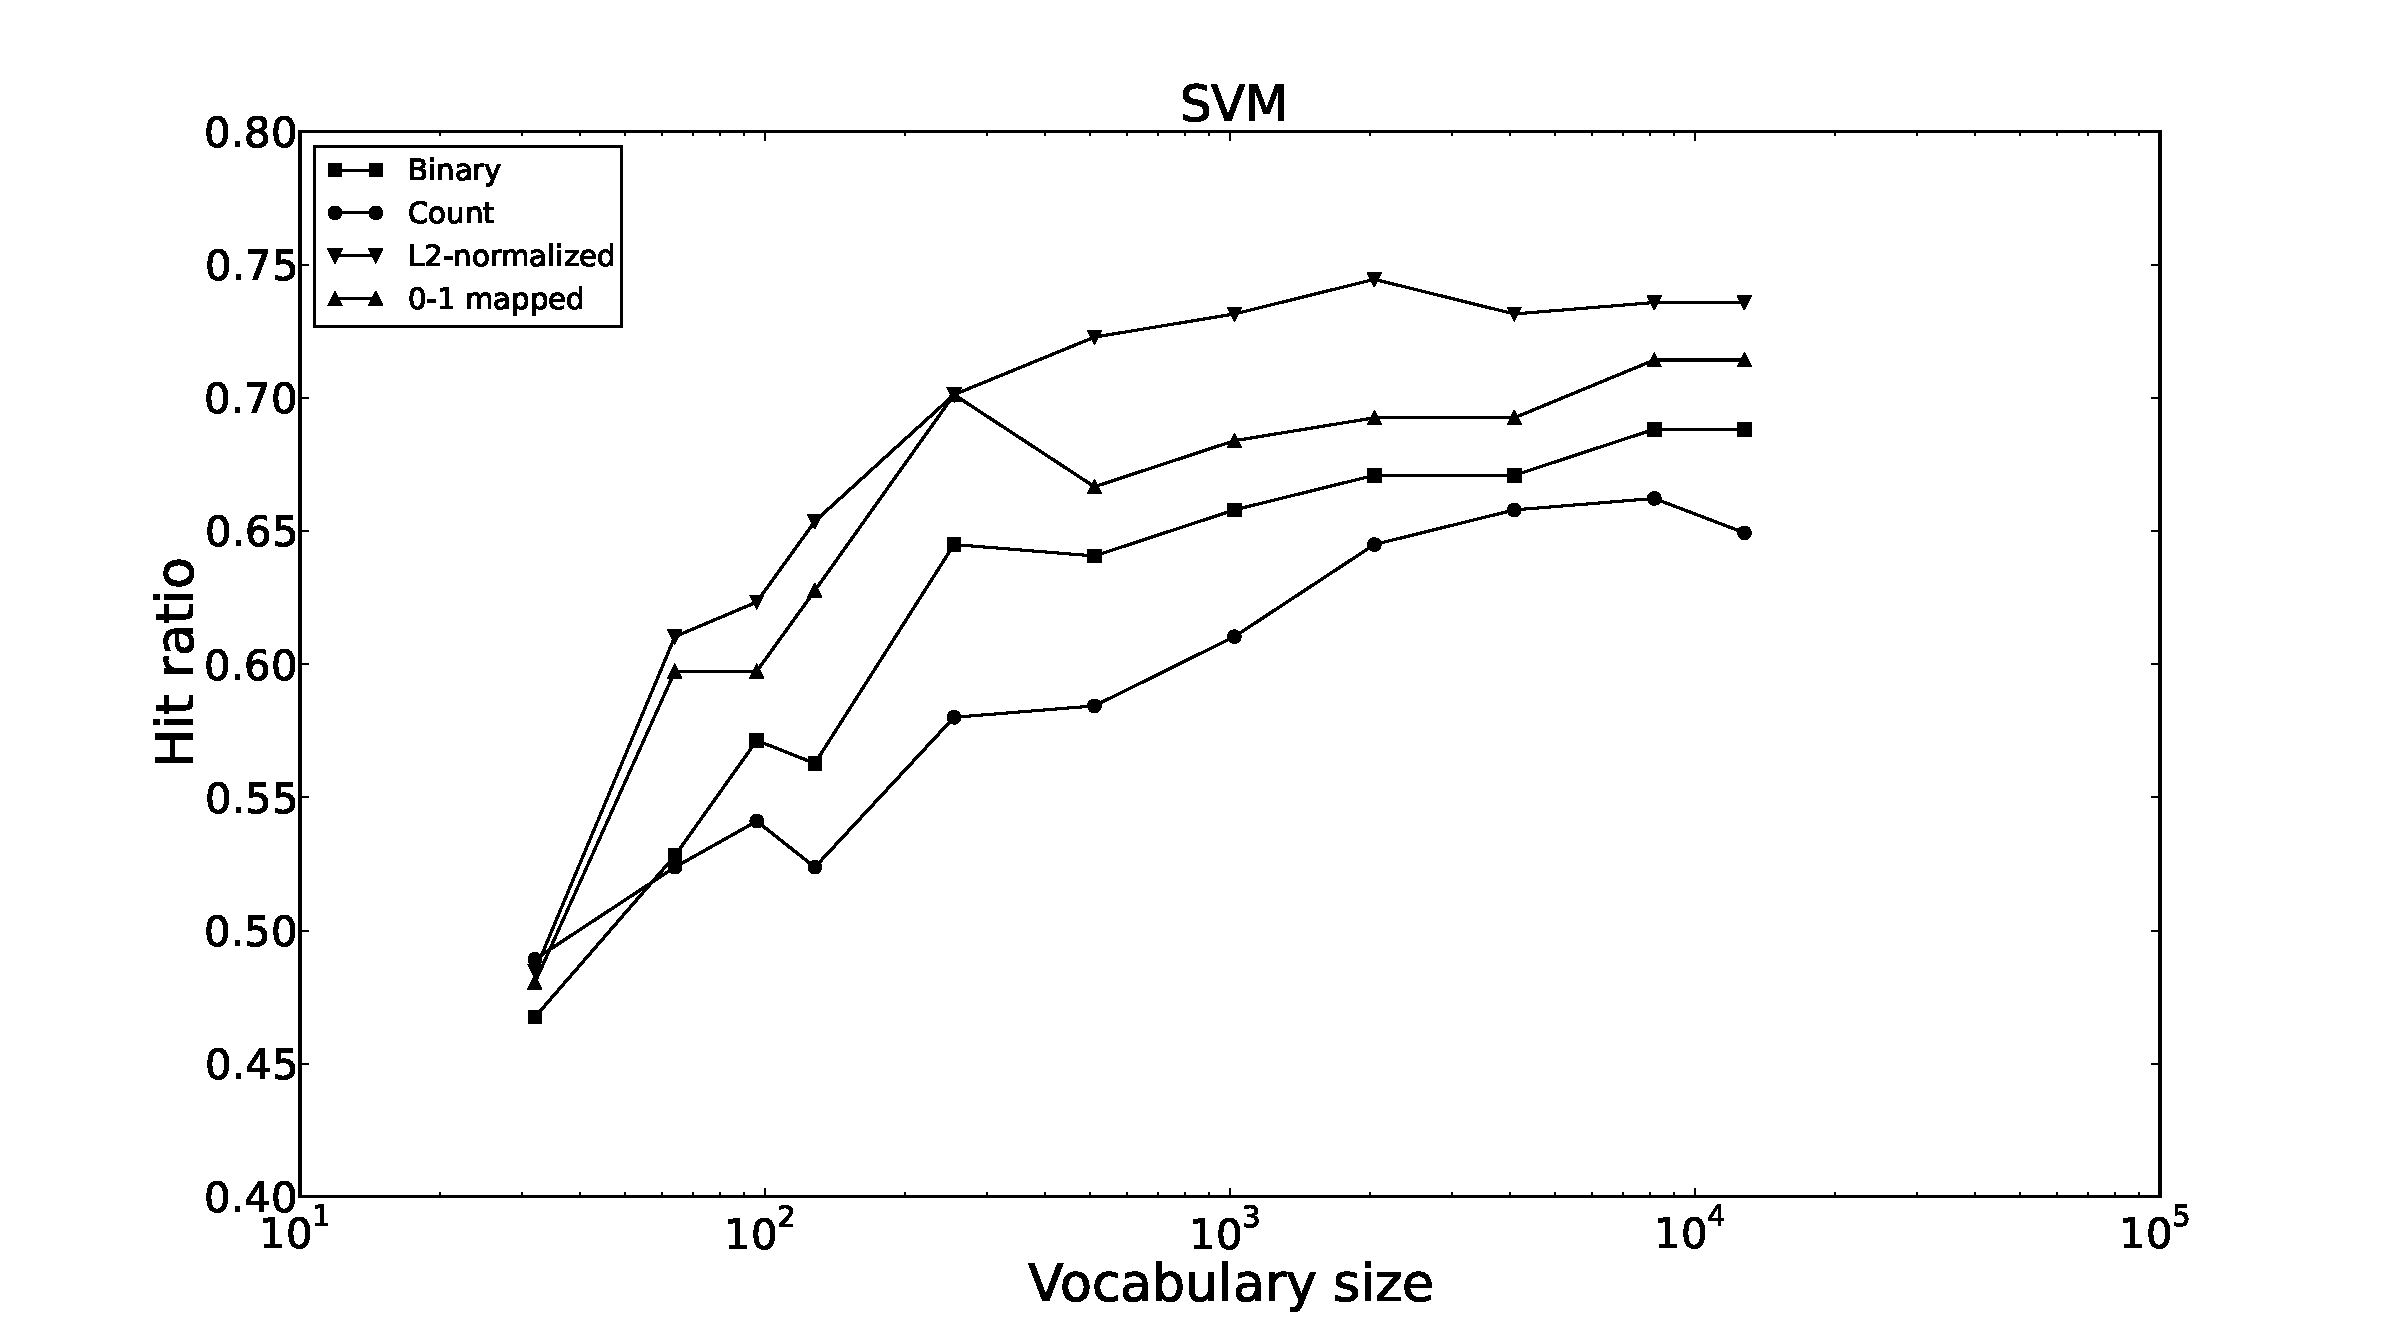
\includegraphics[width=\textwidth]{img/SVM-hitrate-eps-converted-to.pdf}
		\caption{Hit ratio of SVM classifier with varying vocabulary size.}
		\label{fig:hitratio-svm}
	\end{subfigure}
	\\
	\begin{subfigure}[b]{\figwidth}
		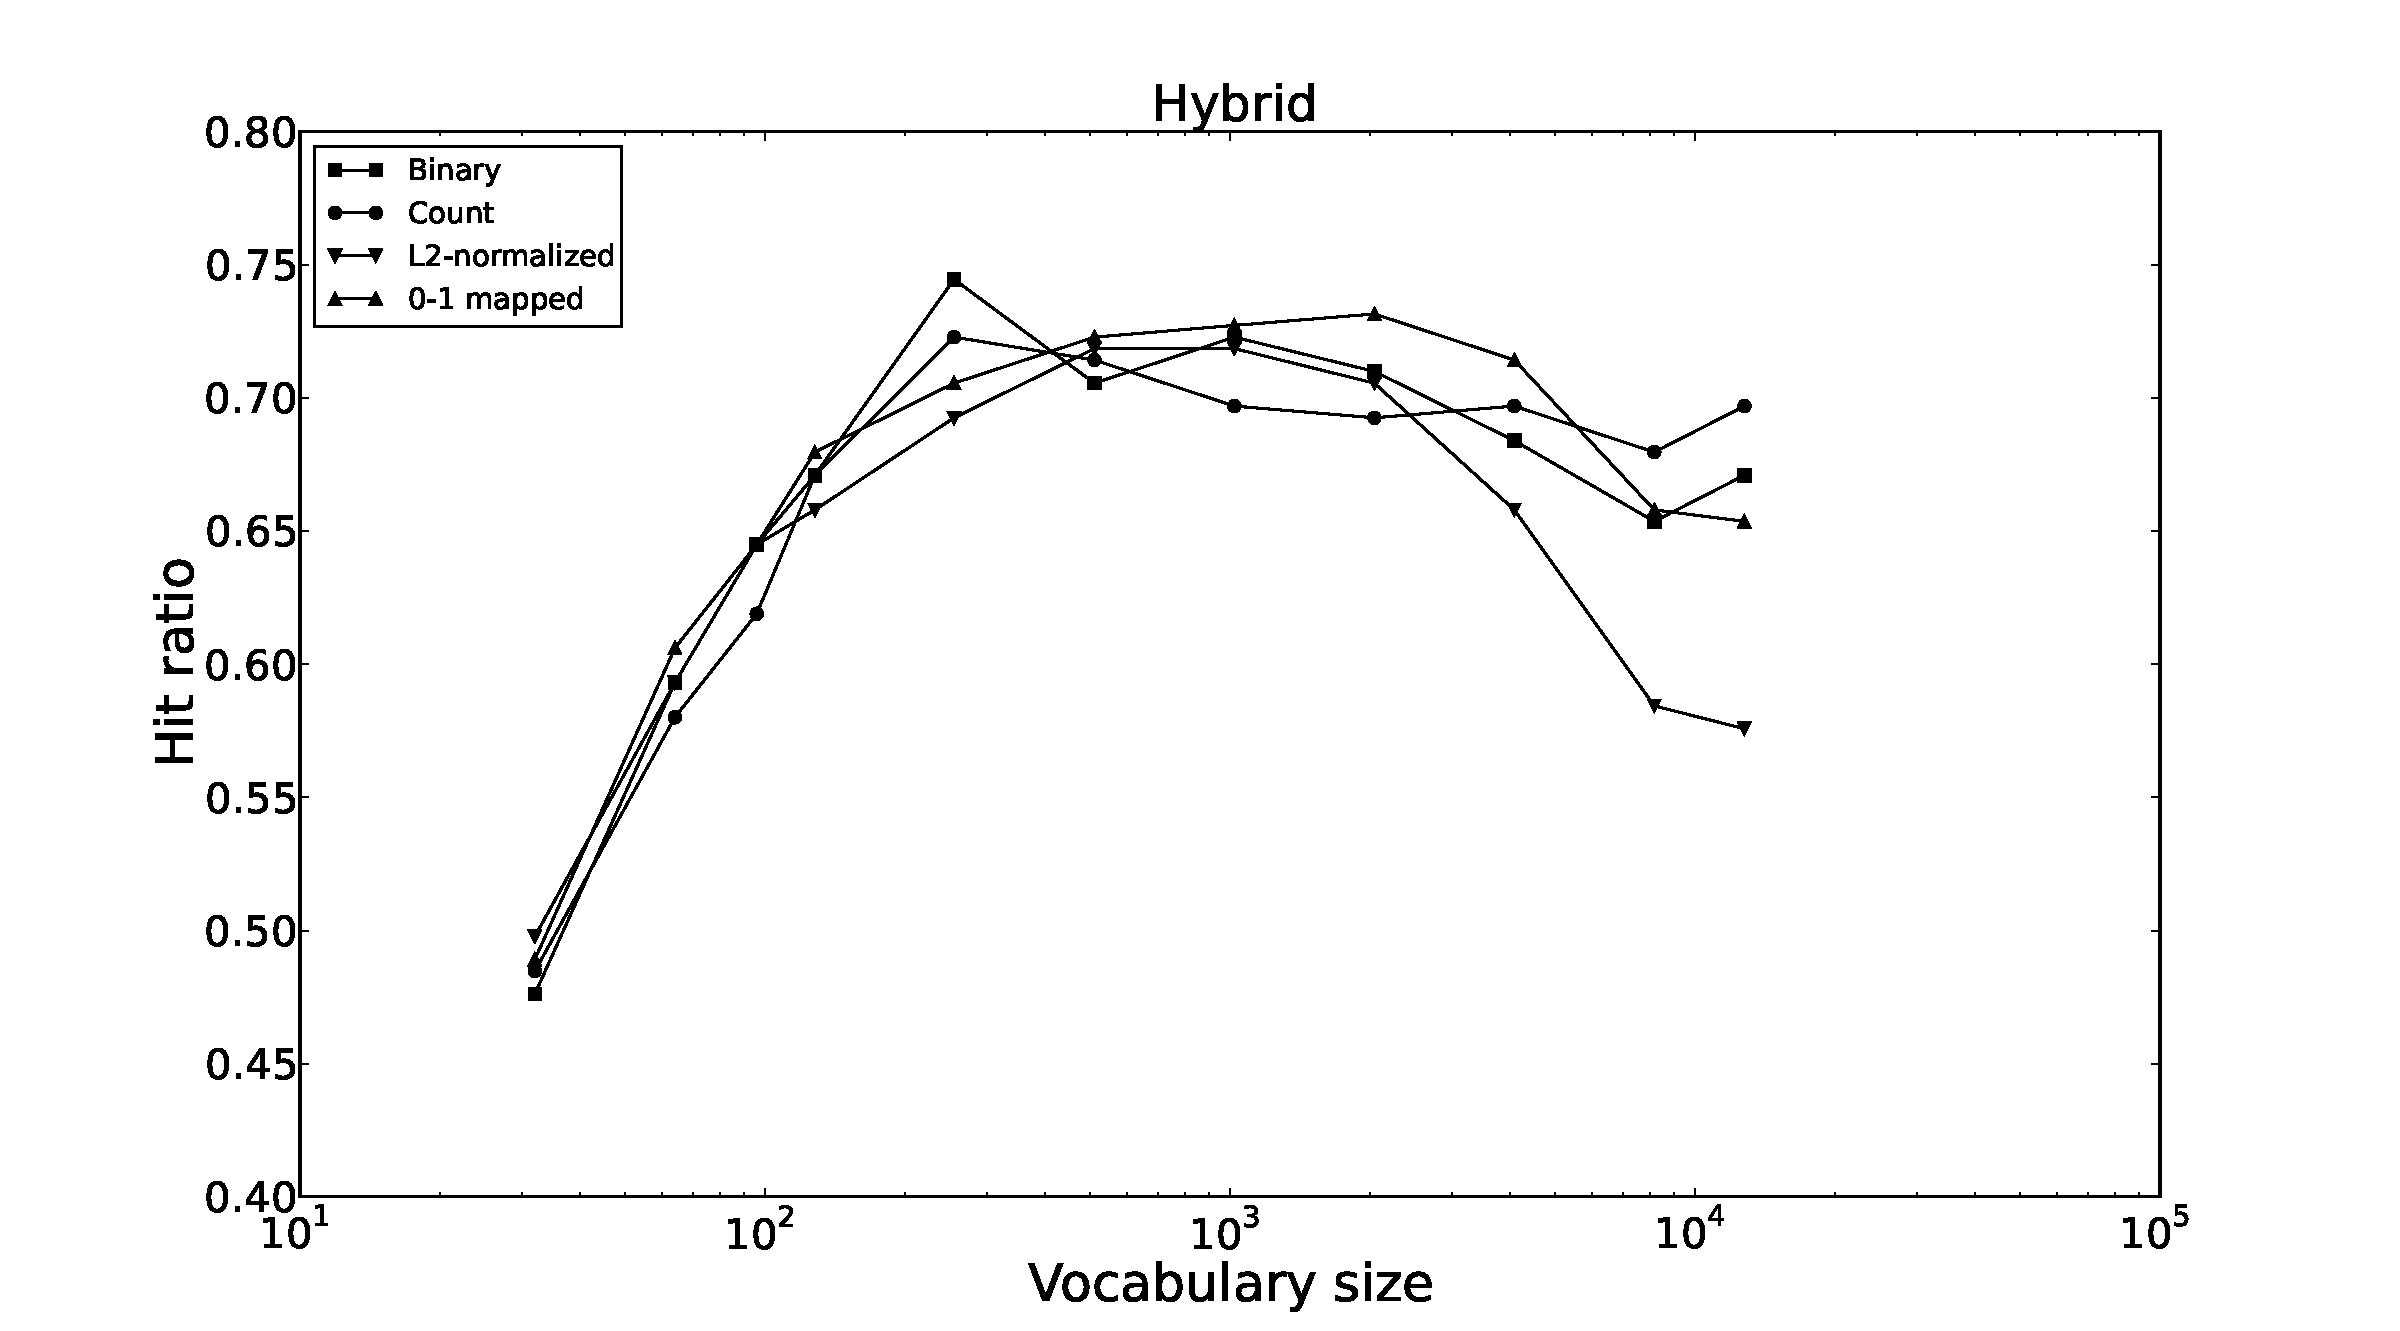
\includegraphics[width=\textwidth]{img/Hybrid-hitrate-eps-converted-to.pdf}
		\caption{Hit ratio of Hybrid classifier with varying vocabulary size.}
		\label{fig:hitratio-hybrid}
	\end{subfigure}
	\caption{Hit ratio vs vocabulary size.}
	\label{fig:hitratio}
\end{figure}

